% !TEX program = xelatex
% Курсовой проект по дисциплине «Разработка профессиональных приложений». Формат XeLaTeX.
\documentclass[14pt,a4paper]{extreport}
\usepackage{timcw}
\begin{document}

% Данные о руководителе заполняются после согласования с кафедрой.
\cwtitle{Приложение для составления и синхронизации списков дел (\mbox{to-do list})}{Галеев Султан Азатович}

\thispagestyle{plain}
\begin{center}
{\small РГАУ-МСХА имени К.\,А. Тимирязева\\
Институт экономики и управления АПК\\
Кафедра статистики и кибернетики}\par\vspace{10mm}
\textbf{ЗАДАНИЕ НА КУРСОВОЙ ПРОЕКТ}
\end{center}
\vspace{5mm}
\noindent Обучающийся: Галеев Султан Азатович\\[4mm]
\noindent Группа: ДЭ 21-25\\[4mm]
\noindent Дисциплина: «Разработка профессиональных приложений».\\[4mm]
\noindent Тема: «Приложение для составления и синхронизации списков дел (to-do list)».\\[4mm]
\noindent Исходные данные: два персональных компьютера, одна локальная сеть, язык Python, приложение с графическим интерфейсом, база SQLite.\\[4mm]
\noindent Необходимо разработать: создание и редактирование задач, изменение отметки выполнения, поиск и фильтрацию записей, страницу статистики, сохранение списка в текстовый файл, сервер обмена данными и проверку работы двух клиентов.\\[4mm]
\noindent Материалы к защите: исходные файлы проекта, пояснительная записка, схемы операций, снимки интерфейса, схемы работы приложения и результаты проверки запросов.\\[12mm]
\noindent Дата выдачи задания: \rule{58mm}{0.4pt}\\[8mm]
\noindent Руководитель: \rule{87mm}{0.4pt}\\[8mm]
\noindent Задание принял: \rule{84mm}{0.4pt}
\vfill

\clearpage

\thispagestyle{plain}
\begin{center}\textbf{АННОТАЦИЯ}\end{center}

В курсовом проекте рассмотрено приложение для ведения общего списка задач на двух персональных компьютерах. В графическом окне можно добавить задачу, исправить её название, изменить отметку о выполнении или удалить запись. Предусмотрены поиск по названию, фильтр по состоянию, страница со статистикой и сохранение списка в TXT. Оба компьютера используют один клиент PySide6, подключённый к серверу в локальной сети.

Сервер FastAPI принимает запросы и обращается к базе SQLite. Задачи хранятся в одной таблице, поэтому изменения доступны с обоих устройств. Клиент запрашивает список каждые две секунды и обновляет окно, когда данные изменились. Работа без соединения с сервером не предусмотрена.

Структура базы данных включает идентификатор, название и отметку выполнения задачи. Для обмена данными используются пять HTTP-маршрутов. Алгоритмы добавления, изменения и обновления задач представлены блок-схемами. Работа графического интерфейса и двух экземпляров клиента на одном компьютере показана на снимках экрана. Проверка двух физических компьютеров описана отдельно и не считается проведённой.

\noindent\textbf{Ключевые слова:} Python, PySide6, FastAPI, SQLite, список дел, синхронизация, настольное приложение.
\clearpage

\tableofcontents
\clearpage

\intro
При работе на домашнем и учебном компьютерах один и тот же список заданий приходится поддерживать на двух устройствах. Если записи хранятся отдельно, на одном ПК задача может быть уже выполнена, а на другом по-прежнему отображаться как незавершённая. Общая база позволяет видеть одни и те же задачи на обоих компьютерах.

В проекте разрабатывается настольное приложение для двух ПК. Каждый компьютер запускает графическое окно, в котором можно добавлять, исправлять, искать и отмечать задачи. Оба окна отправляют запросы одному серверу, который сохраняет задачи в базе SQLite. После изменения данных на одном компьютере второй получает новое состояние при следующем обновлении.

Программа рассчитана на два персональных компьютера в одной локальной сети. Для обоих устройств используется один настольный клиент. Сервер и файл базы данных располагаются на первом компьютере.

\textbf{Цель курсового проекта}: создать приложение для ведения общего списка задач с графическим интерфейсом, базой данных SQLite и синхронизацией между двумя ПК через локальную сеть.

Для достижения цели необходимо определить операции пользователя, создать таблицу базы данных, написать обработчики запросов, собрать интерфейс с тремя страницами и проверить обмен изменениями между двумя клиентами. Отдельно рассматриваются неправильный ввод и отсутствие сетевого соединения.

\textbf{Объект проекта}: общий список дел. \textbf{Предмет проекта}: хранение задач и передача изменений между двумя персональными компьютерами.

Графический интерфейс разработан на PySide6, HTTP-запросы обрабатывает FastAPI, а данные хранятся в SQLite. Взаимодействие этих компонентов позволяет изменять общий список задач из двух независимых окон.

\chapter{Проектирование приложения для общего списка дел}

\section{Предметная область и назначение программы}

Списки дел используются для записи учебных заданий, покупок, личных планов и других предстоящих дел. Для каждой задачи хранятся идентификатор, название и отметка выполнения. Например, задачу «Сдать практическую работу» можно добавить в общий перечень и отметить выполненной после завершения. Даты, приоритеты, категории и повторяющиеся события в рассматриваемую модель не входят. Для двух компьютеров достаточно общего перечня задач и отметок об их выполнении.

Пользователь может работать на двух компьютерах. При локальном хранении на каждом устройстве возникли бы два независимых списка. Даже если файлы имеют одинаковую структуру, они со временем расходятся: на одном компьютере задача отмечена выполненной, а на втором об этом ещё неизвестно. При ручном копировании файлов нужно отдельно следить, какая версия списка последняя. Список хранится в SQLite на первом компьютере; оба клиента обращаются к нему через FastAPI.

Приложение рассчитано на локальную сеть, например домашнюю или учебную. Один компьютер запускает сервер и хранит данные. Второй компьютер является клиентом. При этом на первом компьютере тоже можно запустить клиент, поэтому у обоих пользователей будет одинаковый интерфейс. Сведения о задачах передаются по HTTP в виде JSON-документов. Клиент отправляет запрос, сервер возвращает ответ; такой обмен описан в русскоязычном руководстве MDN \cite{mdnhttp}. JSON представляет данные в виде объектов, массивов и значений разных типов \cite{rfcjson}. В ответе сервера передаются идентификатор, название и состояние задачи.

Основу серверного интерфейса составляют чтение списка, добавление записи, исправление её названия, переключение отметки и удаление. После каждой операции данные остаются в одной базе. Сервер отвечает за проверку запроса и изменение нужной строки, а клиенты - за отображение результата. Такой способ хранения позволяет работать с задачами по идентификатору, даже если две записи имеют одинаковое название.

Сохранение данных и синхронизация проверяются раздельно. Сохранение означает, что запись остаётся в SQLite после перезапуска сервера. Синхронизация означает, что изменение с одного компьютера получает второй клиент. Если задача видна на другом ПК, но исчезает после перезапуска сервера, обмен данными работает, а сохранение данных не работает. Поэтому отдельно проверяются чтение общей базы и повторный запуск с тем же файлом данных.

У программы есть несколько допущений. Компьютеры используют доверенную локальную сеть; в приложении нет личных аккаунтов. Пользователи видят один список, а не личные списки каждого. Клиенты подключаются к серверу по его локальному IP-адресу. Если компьютер-сервер выключен, клиент сохраняет на экране ранее полученный список, но не обновляет его. Нижняя строка сообщает об отсутствии связи; отправка новой команды завершится ошибкой.

\section{Пользовательские действия и требования}

Функции приложения определены по последовательности действий пользователя. При составлении требований учитываются действия, исходные данные и ожидаемый результат операции; такой способ описания используется при проектировании информационных систем \cite{zaramenskikh,chistov}. После открытия приложения пользователь видит список задач. Он может создать новую запись, исправить название, отобрать записи по тексту или состоянию, а также отметить выполнение. Для удаления требуется выбрать конкретную строку. Второй компьютер должен показывать тот же перечень, хотя обновление может произойти с небольшой задержкой. Эти действия сформировали набор функциональных требований, приведённый в таблице \ref{tab:req-functional}.

\begin{table}[H]
\caption{Функциональные требования к приложению}
\label{tab:req-functional}
\small\centering\renewcommand{\arraystretch}{1.25}
\begin{tabularx}{\textwidth}{|L{13mm}|Y|L{33mm}|}
\hline
Код & Требование & Проверяемый результат \\
\hline
F1 & Показать актуальный перечень задач & Виден список записей \\
\hline
F2 & Добавить задачу с непустым названием & Новая запись появилась \\
\hline
F3 & Изменить отметку о выполнении & Состояние поменялось \\
\hline
F4 & Удалить выбранную задачу & Запись исчезла \\
\hline
F5 & Передать изменения второму клиенту & Список на ПК №2 обновился \\
\hline
F6 & Сохранить задачи после перезапуска & Список остался в базе \\
\hline
F7 & Обработать неверный ввод & Ошибочная запись не создана \\
\hline
F8 & Показать проблему соединения & Пользователь видит сообщение \\
\hline
F9 & Перейти между тремя страницами & Переключается раздел интерфейса \\
\hline
F10 & Исправить название существующей задачи & Новое название сохранено \\
\hline
F11 & Найти задачи и применить фильтр & Видны подходящие записи \\
\hline
F12 & Посчитать выполненные задачи & Показаны числа и процент \\
\hline
F13 & Сохранить список в TXT & Создан текстовый файл со всеми задачами \\
\hline
\end{tabularx}
\end{table}

Ввод названия задачи ограничен 120 символами. То же правило действует при редактировании. Сервер проверяет текст независимо от клиентского окна, поскольку запрос можно отправить и напрямую через страницу документации API. Название проверяется после удаления пробелов по краям строки; длина должна составлять от 1 до 120 символов. Управляющие символы (например, перевод строки и табуляция) сервер отклоняет: название должно отображаться одной строкой списка \cite{owaspvalidation}.

Признак выполнения принимает два значения. В интерфейсе выполненная задача отмечается знаком [x], невыполненная: знаком [ ]; при передаче по сети используется логическое значение. В списке не нужно выводить техническое значение поля \texttt{done}. Название записи остаётся одинаковым независимо от состояния. Повторное изменение переводит задачу из состояния «Выполнено» обратно в «В работе».

При редактировании название меняется только у выбранной записи; её идентификатор и отметка выполнения сохраняются. Поиск и фильтрация выполняются над уже полученным списком на клиенте и не изменяют содержимое базы данных. Кнопка «Сохранить в TXT» записывает все задачи в текстовый файл на компьютере пользователя; отдельный маршрут на сервере для этого не нужен. Для удаления пользователь должен выбрать строку списка. Если ни одна строка не выбрана, интерфейс показывает подсказку. На уровне сервера удаление выполняется по идентификатору. Когда такого идентификатора нет, сервер отвечает кодом 404, не изменяя другие записи. Это позволяет отделить отсутствие задачи от успешно проведённой операции. Семантика ошибок HTTP и назначение кодов ответа описаны в стандарте HTTP \cite{rfchttp}.

Нефункциональные требования касаются установки, работы с сетью и отображения ошибок. Программа должна запускаться без внешней учётной записи, а для хранения данных не должна требоваться установка отдельного серверного процесса базы данных. Все основные действия располагаются в одном окне. Для всех сетевых запросов установлен тайм-аут 2 секунды. Запросы выполняются в графическом потоке, поэтому при задержке сети окно может на короткое время перестать отвечать. Перечень нефункциональных требований приведён в таблице \ref{tab:req-nonfunctional}. 

\begin{table}[H]
\caption{Нефункциональные требования и ограничения}
\label{tab:req-nonfunctional}
\small\centering\renewcommand{\arraystretch}{1.25}
\begin{tabularx}{\textwidth}{|L{17mm}|Y|}
\hline
Код & Содержание \\
\hline
N1 & Оба клиента имеют одинаковую функциональность и интерфейс \\
\hline
N2 & Данные хранятся в одной базе на компьютере-сервере \\
\hline
N3 & Рабочая сеть локальная; доступ в публичный интернет не требуется \\
\hline
N4 & Интерфейс показывает проблемы ввода и соединения понятным текстом \\
\hline
N5 & Проект устанавливается средствами Python и одного файла зависимостей \\
\hline
N6 & Автоматическое обновление списка происходит раз в 2 секунды \\
\hline
N7 & При демонстрации доступ к серверу ограничен доверенной локальной сетью \\
\hline
\end{tabularx}
\end{table}

Для функциональных требований определены проверяемые сценарии. Для F2 достаточно создать новую запись и проверить её наличие. Для F5 нужны два клиента, подключённые к одной базе. Для F6 сервер перезапускается с тем же файлом SQLite. Для F7 отправляется пустое название, для F10 проверяется исправление названия с сохранением прежнего идентификатора. Работа поиска, фильтра и статистики проверяется в клиентском окне.

В базе нет поля с именем пользователя: любые изменения относятся к общему списку. Клиент поэтому не показывает форму входа и не разделяет задачи на личные и чужие.

\section{Выбор инструментов}

Приложение разделено на клиентскую и серверную части. На клиенте выполняется графический интерфейс. Сервер принимает запросы двух клиентов и работает с общей базой данных. Обе части написаны на Python. Для обработки запросов, работы с интерфейсом и обращения к базе применяются библиотеки этого языка. Для обработки строк, списков и функций используются обычные средства Python; их применение рассматривается в учебном пособии по Python 3 \cite{polupanov}. Доступ к SQLite предоставляется стандартным модулем \texttt{sqlite3} \cite{pythonsqlite}.

Для интерфейса используется PySide6, официальный набор привязок Qt для Python. С его помощью можно создавать окно, текстовое поле, кнопки, список и разные страницы без написания HTML или JavaScript. Окно и его страницы построены из стандартных элементов Qt. В пособии Н.\,А. Прохоренка и В.\,А. Дронова рассматривается создание окон и обработка событий в Qt; в данной работе использованы привязки PySide6, для которых доступна отдельная документация \cite{prokhorenok,qtdocs}. В окне задействованы поле ввода, список, кнопки, выпадающий фильтр, индикатор выполнения и три страницы.

Одинаковый исходный код клиента PySide6 запускается на компьютерах с Windows. Оба клиента обращаются к общему серверу по локальной сети. Каждый клиент запрашивает данные самостоятельно, поэтому изменения списка передаются через сервер без копирования файлов базы данных.

Серверная часть построена на FastAPI. Схема обмена запросами соответствует клиент-серверному подходу, рассматриваемому в учебной литературе по веб-программированию на Python \cite{yantsev}. В данном проекте клиентом выступает окно PySide6, а не браузер. В FastAPI обработчик связывается с HTTP-методом и адресом. Клиент может запросить список задач по одному адресу, а создать новую задачу по другому. FastAPI автоматически формирует описание API и интерактивную страницу документации. Встроенная страница документации позволяет просмотреть доступные операции и вручную выполнить запрос к серверу \cite{fastapifirst}.

Для передачи данных применён JSON. Запрос создания задачи содержит название. Ответ на чтение списка содержит идентификатор, текст и отметку выполнения каждой задачи. Тело запроса и ответа можно просмотреть в интерактивной документации FastAPI. FastAPI позволяет описать структуру тела запроса через модели данных, после чего проверяет типы перед вызовом обработчика \cite{fastapibody}. На стороне Python для такой проверки используется Pydantic. Проверка названия выполняется при добавлении и редактировании: пробелы по краям удаляются, пустая строка отклоняется.

Для хранения задач используется SQLite. Это файловая база данных, с которой Python работает через встроенный модуль \texttt{sqlite3}. Файл базы находится на компьютере с FastAPI. Отдельный сервер СУБД не нужен. В проекте одна таблица с названиями и состояниями задач. SQL-запросы выполняются с параметрами вместо подстановки введённого пользователем текста. Такой способ не требует ручного экранирования ввода \cite{pythonsqlite}. Назначение технологий указано в таблице \ref{tab:stack}.

\begin{table}[H]
\caption{Назначение использованных технологий}
\label{tab:stack}
\small\centering\renewcommand{\arraystretch}{1.23}
\begin{tabularx}{\textwidth}{|L{34mm}|Y|}
\hline
Инструмент & Роль в системе \\
\hline
Python & Общий язык клиентской и серверной частей \\
\hline
PySide6 & Окно с тремя страницами, поиск, фильтр и индикатор выполнения \\
\hline
FastAPI & Маршруты запросов, проверка входных данных, документация API \\
\hline
SQLite & Хранение задач в файле на компьютере-сервере \\
\hline
Requests & Отправка HTTP-запросов из настольного клиента \\
\hline
HTTP и JSON & Передача запросов и данных между клиентами и сервером \\
\hline
\end{tabularx}
\end{table}

Для отправки запросов из настольного клиента используется Requests. В этой библиотеке есть методы для обычных HTTP-операций и возможность устанавливать время ожидания. При ошибках соединения или при ответе сервера с кодом ошибки вызываются исключения. По полученному исключению клиент различает успешный запрос и сбой связи \cite{requestsquick}. Для проверки серверных запросов применялся TestClient из набора средств FastAPI \cite{fastapitesting}.



\section{Архитектура и обмен данными}

На рисунке \ref{fig:architecture} показаны два компьютера. На первом работают сервер FastAPI и клиент PySide6, на втором - только клиент. Оба клиента обращаются к одному адресу сервера, который выполняет операции с файлом SQLite. Клиентам не требуется открывать базу данных через сетевую папку.

\begin{figure}[H]
\centering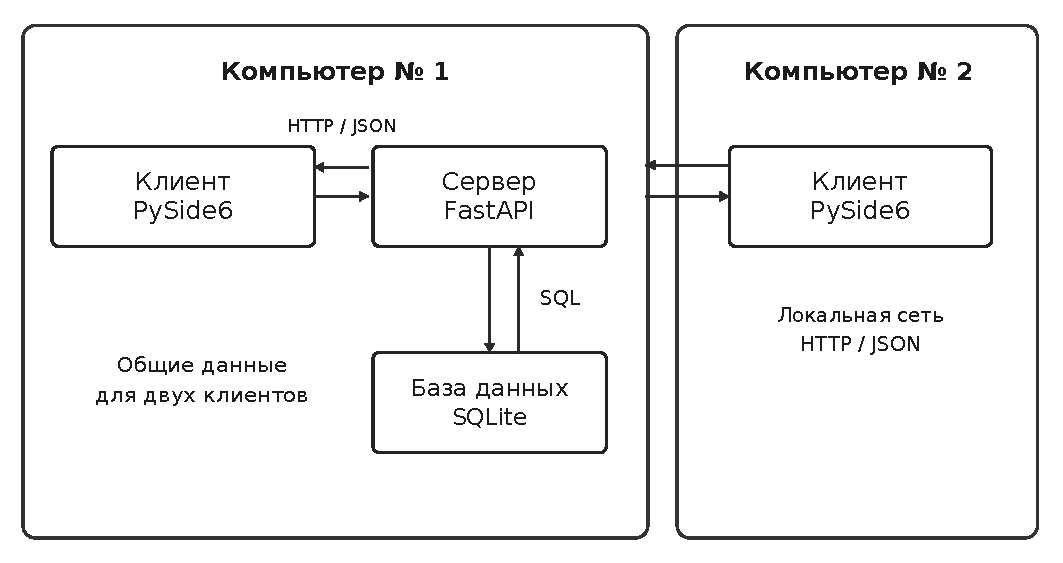
\includegraphics[width=.94\textwidth]{figures/arch.pdf}
\caption{Взаимодействие двух клиентов, сервера и базы данных}
\label{fig:architecture}
\end{figure}

Действие пользователя проходит несколько этапов. Например, при добавлении задачи клиент получает текст из поля ввода. Если введены только пробелы, сообщение об ошибке показывается сразу, без обращения к серверу. Если ввод корректный, клиент отправляет POST-запрос. Сервер ещё раз проверяет название, выполняет вставку в SQLite, сохраняет изменение и отправляет ответ об успехе. После ответа клиент запрашивает обновлённый список. Второй компьютер увидит эту запись после следующего запроса обновления.

При изменении состояния сначала выбирается конкретная строка. Из её данных извлекается целочисленный идентификатор, а затем отправляется PATCH-запрос по её идентификатору. Сервер переключает отметку выполнения соответствующей записи. Если запись уже отсутствует, сервер возвращает HTTP 404. Клиент показывает предупреждение «Не удалось выполнить действие» и повторно запрашивает список. Тот же принцип используется при удалении: операция выполняется только для существующего идентификатора. Смысл используемых методов и кодов ответа соответствует общим правилам HTTP \cite{rfchttp}.

Для синхронизации выбран периодический опрос сервера. В каждом клиенте таймер срабатывает один раз в две секунды и запускает получение списка задач. Полученный список сравнивается с предыдущим. Если изменений нет, интерфейс остаётся таким же. Если данные отличаются, список заполняется заново. Применение таймера для периодических действий предусмотрено библиотекой Qt \cite{qtimer}. Постоянное соединение с сервером для этого алгоритма не используется.

Изменение появляется на втором ПК при следующем запросе таймера, поэтому обновление не происходит мгновенно. Если компьютер-сервер недоступен, клиент показывает ошибку и не сохраняет отправленную команду локально. После восстановления соединения очередной запрос возвращает актуальный список SQLite. Измерение оптимального интервала опроса не проводилось.

При одновременной работе двух пользователей возможны ситуации, когда один удаляет задачу, а второй пытается изменить её состояние. Проверка количества изменённых строк на сервере позволяет отличить несуществующую запись от существующей. В таком случае клиент получает 404. Правила сложного разрешения конфликтов не требуются: все изменения проходят через одну таблицу и выполняются как отдельные операции. Но приложение не фиксирует историю действий, поэтому после удаления нельзя восстановить прежнее состояние средствами самой программы.

\section{Структура базы данных и интерфейса}

Задачи хранятся в таблице \texttt{tasks}. В неё входят идентификатор, название, отметка выполнения. Идентификатор формируется автоматически и позволяет выбрать нужную запись при изменении или удалении. Название хранится как текст. Признак выполнения записывается как число 0 или 1, но в передаваемом JSON преобразуется в логическое значение. Отдельного поля владельца задачи нет, поскольку список общий.

SQLite позволяет создавать таблицу с первичным ключом и ограничениями на отсутствие значения NULL. В таблице нет внешних ключей: каждая запись содержит все данные, необходимые клиенту. Операция создания таблицы выполняется при запуске сервера, причём используется вариант с проверкой существования таблицы. Если файл базы уже содержит данные, повторный запуск не должен удалять их. Синтаксис создания таблицы и назначение первичного ключа описаны в документации SQLite \cite{sqlitecreate}. Состав полей приведён в таблице \ref{tab:dbfields}.

\begin{table}[H]
\caption{Поля таблицы tasks и их смысл}
\label{tab:dbfields}
\small\centering\renewcommand{\arraystretch}{1.25}
\begin{tabularx}{\textwidth}{|L{25mm}|L{33mm}|Y|}
\hline
Поле & Тип & Назначение \\
\hline
id & INTEGER & Уникальный идентификатор записи \\
\hline
title & TEXT & Краткое название задачи \\
\hline
done & INTEGER & 0: в работе, 1: выполнено \\
\hline
\end{tabularx}
\end{table}

Для чтения списка сервер использует запрос SELECT с сортировкой. Новые записи выводятся выше старых, независимо от отметки выполнения. Это правило применяется сервером, поэтому оба клиента получают одинаковый порядок. SQL-операция SELECT предназначена для выбора данных из таблиц и допускает указание порядка результатов \cite{pythonsqlite}.

Изменение состояния выполняется операцией UPDATE, которая меняет поле \texttt{done} только у строки с указанным идентификатором \cite{pythonsqlite}. Удаление реализуется операцией DELETE с таким же условием выбора одной записи \cite{pythonsqlite}. Пользовательский текст передаётся в SQL как параметр, что позволяет безопасно хранить обычные символы, включая кавычки. В коде нет ручного построения SQL-запроса из введённого названия.

В клиенте три страницы (рисунок \ref{fig:navigation}). На первой доступны добавление, поиск, фильтрация, редактирование, изменение статуса, удаление и сохранение списка в TXT. На второй показаны число всех задач, количество выполненных и индикатор доли выполнения. Третья содержит сведения о программе и адрес сервера. Переключение выполняется вкладками в верхней части окна.

\begin{figure}[htbp]
\centering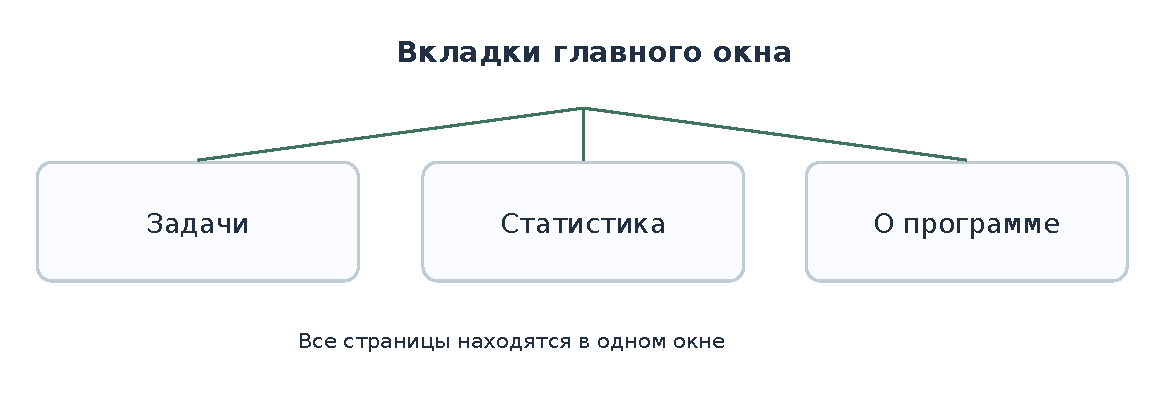
\includegraphics[width=.92\textwidth]{figures/nav.pdf}
\caption{Переход между страницами приложения}
\label{fig:navigation}
\end{figure}

Для переключения трёх страниц используется QTabWidget \cite{qttabs}. Список построен на QListWidget: у каждой строки отдельно сохраняется идентификатор задачи. Кнопка «Изменить» открывает стандартный диалог ввода текста; двойной щелчок по строке меняет отметку выполнения \cite{qtlist}. Поиск сравнивает названия без учёта регистра, а фильтр оставляет все задачи, только невыполненные или только выполненные.

В памяти клиента хранится последний полученный список задач. Это позволяет не перестраивать список каждые две секунды без необходимости. При обновлении, которое действительно меняет строки, клиент пытается сохранить выбранную пользователем запись по её идентификатору. Такой механизм нужен, чтобы автоматический опрос не мешал нажимать кнопки. Данные о выбранной строке читаются из специального поля элемента списка, а не извлекаются из видимого текста, который может совпадать у разных задач.

Страница статистики показывает общее число задач, количество выполненных и их процент. Если список пуст, индикатор показывает ноль. Эти показатели вычисляются из полученных клиентом данных, без дополнительных таблиц и запросов к базе. Адрес сервера задаётся при запуске клиента, а не через отдельную страницу настроек.

\chapter{Реализация и проверка приложения}

\section{Состав проекта и запуск}

Серверная часть содержит пять маршрутов HTTP и операции с SQLite. Настольный клиент выводит окно PySide6 и обрабатывает действия пользователя. Для установки библиотек предусмотрен файл зависимостей, для запуска на Windows используются командные файлы \path{START.bat}, \path{SERVER_ONLY.bat} и \path{CLIENT_OTHER_PC.bat}. Состав основных файлов приложения приведён в таблице \ref{tab:project-files}.

\begin{table}[H]
\caption{Основные файлы приложения}
\label{tab:project-files}
\small\centering\renewcommand{\arraystretch}{1.23}
\begin{tabularx}{\textwidth}{|L{53mm}|Y|}
\hline
Файл & Назначение \\
\hline
server.py & Сервер FastAPI и хранение задач в SQLite \\
\hline
client.py & Окно PySide6, список дел и обработка кнопок \\
\hline
requirements.txt & Библиотеки для установки на двух компьютерах \\
\hline
START.bat & Запуск сервера и двух клиентов на одном ПК \\
\hline
SERVER\_ONLY.bat & Запуск сервера на первом ПК \\
\hline
CLIENT\_OTHER\_PC.bat & Запуск клиента на втором ПК \\
\hline
README.txt & Инструкция по запуску \\
\hline
tasks.db & Файл SQLite с общим списком задач; создаётся при первом запуске \\
\hline
\end{tabularx}
\end{table}

На обоих компьютерах устанавливается Python и библиотеки из файла \path{requirements.txt}. На первом ПК командой \path{START.bat} запускаются сервер и два клиента для локальной проверки. Для работы в сети на первом ПК открывают \path{SERVER_ONLY.bat}, а на втором \path{CLIENT_OTHER_PC.bat} и вводят IP-адрес первого компьютера. Сам сервер использует порт 8000. Клиент первого ПК может обращаться к адресу \texttt{127.0.0.1}; второму нужен реальный локальный IPv4-адрес первого ПК.

Чтобы узнать адрес, на первом компьютере достаточно выполнить команду \texttt{ipconfig}. Во время работы оба компьютера должны находиться в одной локальной сети. Если сервер не открывается со второго ПК, нужно проверить адрес и правила брандмауэра Windows. Важно не запускать отдельный сервер на каждом компьютере: иначе программы окажутся подключены к разным базам, и синхронизации не будет.

После запуска сервера рядом с \texttt{server.py} создаётся файл \texttt{tasks.db}, если его ещё нет. В нём сохраняются названия задач и отметки их выполнения. После остановки сервера файл остаётся на диске. Когда сервер запускается снова, он открывает ту же базу. SQLite работает с файлом базы непосредственно, без отдельного сервера СУБД.

\section{Сервер и операции с данными}

Сервер FastAPI обрабатывает пять маршрутов. При чтении он выбирает записи из таблицы \texttt{tasks}; при добавлении вставляет строку; отдельный PATCH-запрос исправляет название, другой PATCH меняет отметку выполнения; DELETE удаляет запись. Перечень операций представлен в таблице \ref{tab:api}.

\begin{table}[H]
\caption{HTTP-операции сервера}
\label{tab:api}
\small\centering\renewcommand{\arraystretch}{1.22}
\begin{tabularx}{\textwidth}{|L{19mm}|L{40mm}|Y|}
\hline
Метод & Адрес & Назначение \\
\hline
GET & /tasks & Получить общий список задач \\
\hline
POST & /tasks & Добавить задачу \\
\hline
PATCH & /tasks/\{id\} & Поменять отметку выполнения \\
\hline
PATCH & /tasks/\{id\}/title & Исправить название задачи \\
\hline
DELETE & /tasks/\{id\} & Удалить выбранную задачу \\
\hline
\end{tabularx}
\end{table}

Для новой задачи клиент передаёт JSON-объект с полем \texttt{title}. FastAPI преобразует данные к модели \texttt{Task}, после чего запускается обработчик добавления \cite{fastapibody}. Он удаляет пробелы по краям и проверяет длину названия. Строка из одних пробелов и название длиннее 120 символов не записываются. Если ввод неверен, сервер возвращает HTTP 400 и сообщение об ошибке. Такая проверка нужна не только графическому окну: запрос может быть отправлен напрямую через страницу \texttt{/docs}.

Данные размещаются в одной таблице SQLite с полями \texttt{id}, \texttt{title}, \texttt{done}. Первичный ключ \texttt{id} генерируется автоматически. При добавлении выполняется SQL INSERT с параметром вместо подстановки пользовательского текста в запрос. Это позволяет хранить строки, содержащие кавычки и другие символы, без ручного формирования SQL-выражения \cite{pythonsqlite}. После сохранения сервер возвращает ответ, а клиент запрашивает обновлённый перечень.

Чтобы исправить название, клиент открывает диалог ввода и отправляет PATCH-запрос на адрес \texttt{/tasks/\{id\}/title}. На сервере применяется та же проверка текста, что при создании задачи. Меняется только поле \texttt{title}; первичный ключ и состояние остаются прежними. Когда пользователь выбирает задачу и нажимает кнопку изменения состояния, приложение отправляет другой PATCH-запрос с идентификатором. Сервер выполняет SQL UPDATE, переключающий число в поле \texttt{done} между 0 и 1. Чтобы изменить именно выбранную запись, используется условие \texttt{WHERE id = ?} \cite{pythonsqlite}. При удалении аналогичным образом выполняется SQL DELETE \cite{pythonsqlite}. Если идентификатор отсутствует, сервер возвращает ошибку HTTP 404.

При чтении списка выполняется запрос SELECT с сортировкой по идентификатору: новые задачи располагаются первыми. В ответе каждая запись содержит целочисленный идентификатор, название и логическую отметку выполнения. Клиент использует эти значения при построении списка. Ему не требуется знать расположение файла базы данных или выполнять SQL-запросы самостоятельно.

Блок \texttt{with sqlite3.connect} автоматически завершает транзакцию: сохраняет изменения при успешной операции и откатывает их при ошибке.

\section{Алгоритмы работы программы}

Алгоритм добавления задачи начинается с пользовательского ввода. После нажатия кнопки выполняется проверка названия. Пустую строку нельзя передать серверу как корректную задачу. Для остальных строк отправляется HTTP-запрос. Если соединение недоступно или сервер отвечает ошибкой, интерфейс сообщает об этом пользователю, не очищая введённый текст. При успешном ответе поле ввода очищается, затем выполняется чтение актуального списка. Последовательность приведена на рисунке \ref{fig:addtask}.

\begin{center}
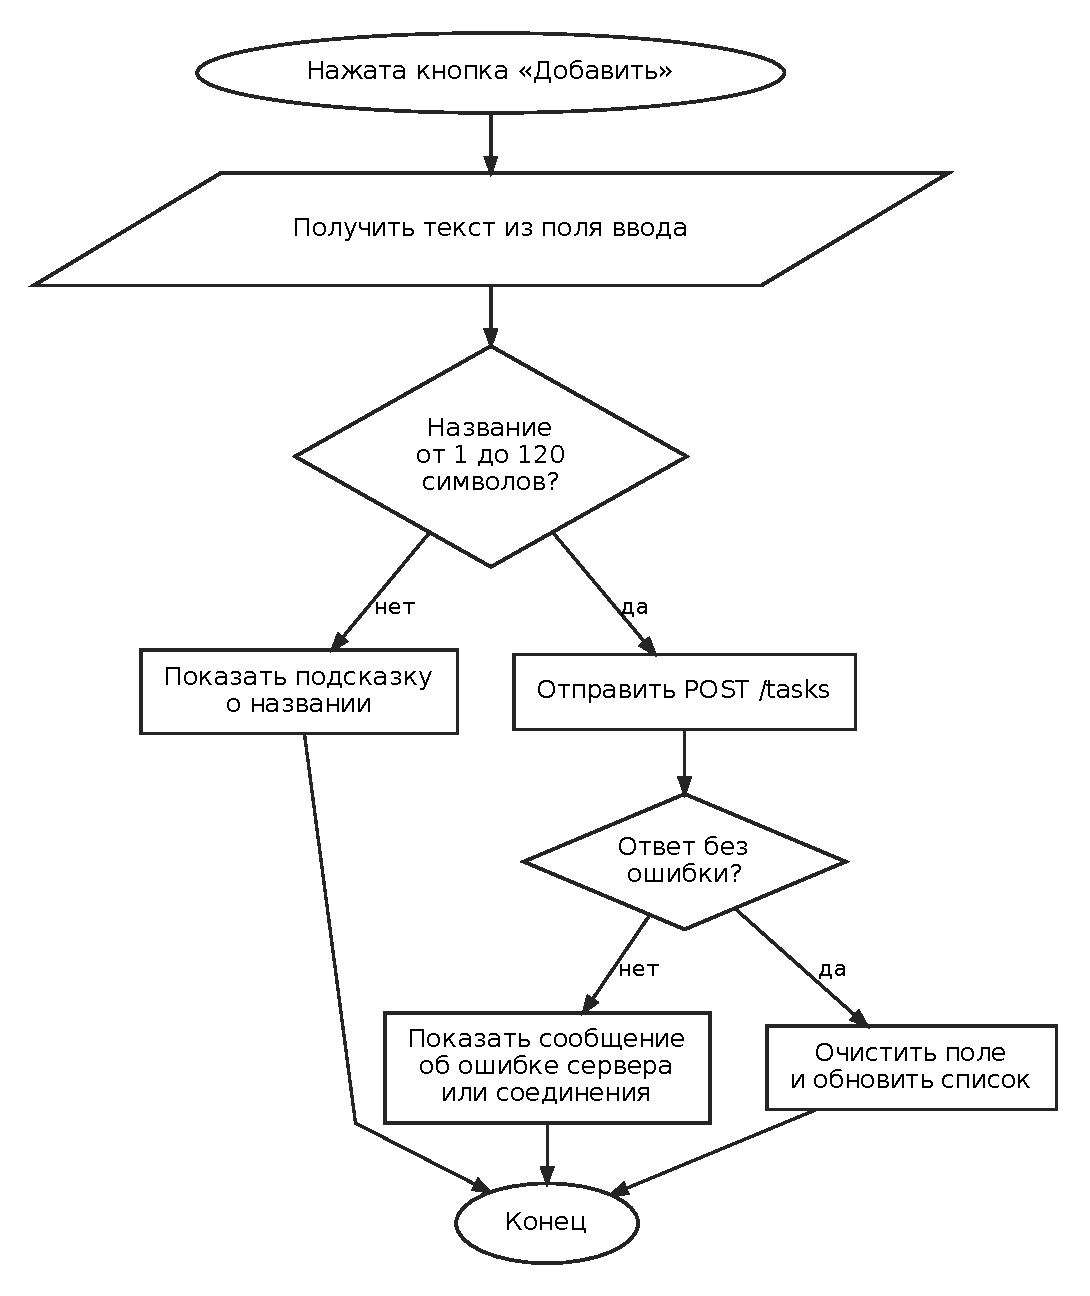
\includegraphics[width=.88\textwidth,height=.58\textheight,keepaspectratio]{figures/add.pdf}
\captionof{figure}{Последовательность добавления задачи и обработки ошибки}
\label{fig:addtask}
\end{center}

На блок-схемах эллипс обозначает начало и конец алгоритма, прямоугольник обозначает действие, а ромб обозначает проверку условия \cite{gostflow}. Ветви ошибки заканчиваются сообщением пользователю без добавления записи.

Редактирование названия показано на рисунке \ref{fig:edit}. Если задача не выбрана, пользователь получает подсказку. Нажатие «Отмена» закрывает диалог без изменений. Название проверяется перед отправкой PATCH-запроса; после успешного ответа клиент получает обновлённый список.

\begin{center}
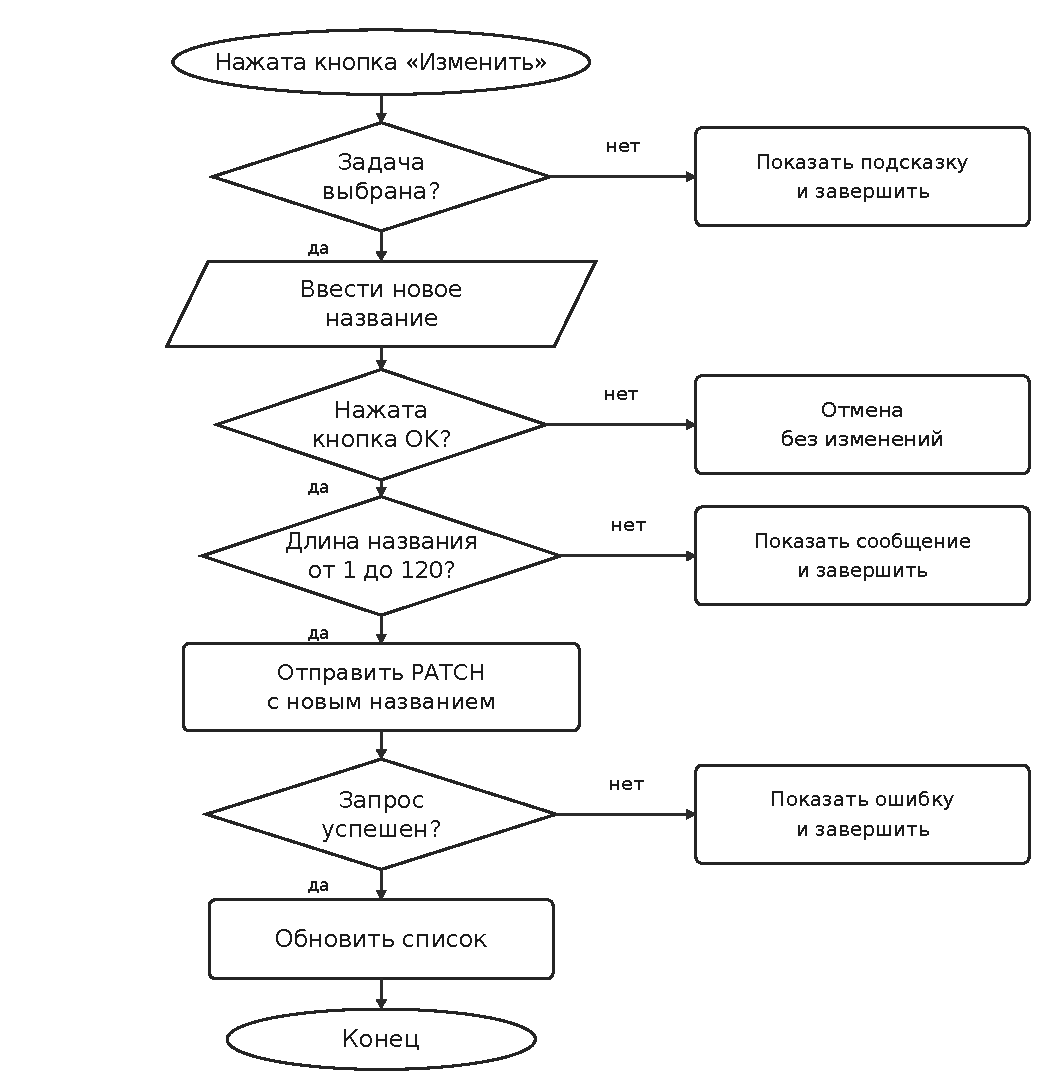
\includegraphics[width=.96\textwidth,height=.65\textheight,keepaspectratio]{figures/edit.pdf}
\captionof{figure}{Алгоритм изменения названия задачи}
\label{fig:edit}
\end{center}

Работа таймера показана на рисунке \ref{fig:sync}. Раз в две секунды клиент запрашивает список. Если данные изменились, он обновляет перечень и показатели статистики; иначе оставляет экран без изменений. Если чтение не удалось из-за отсутствия соединения, нижняя строка сообщает о потере связи. Ранее полученные записи остаются видимыми. При следующем срабатывании таймера запрос повторяется.

\begin{center}
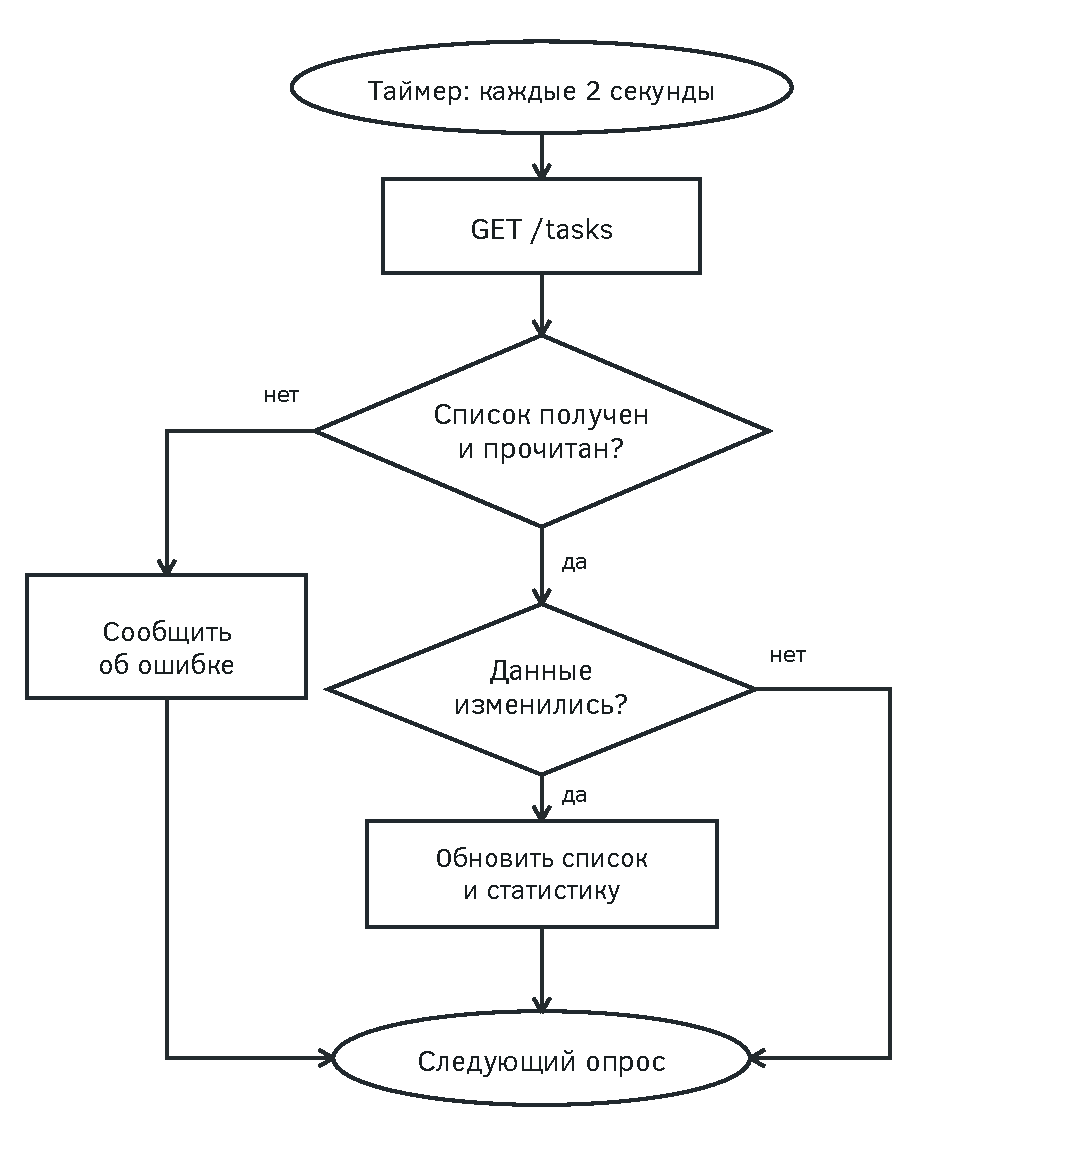
\includegraphics[width=.88\textwidth,height=.58\textheight,keepaspectratio]{figures/sync.pdf}
\captionof{figure}{Алгоритм периодического обновления списка задач}
\label{fig:sync}
\end{center}

Выбранная схема не требует отдельного канала уведомлений от сервера. Оба клиента сами обращаются за актуальными данными. У такого способа есть ограничение: фактическое появление изменения зависит от момента следующего опроса. Если задача была создана непосредственно после очередного запроса второго клиента, он увидит её только при следующем обращении. Таймер настроен на две секунды. Производительность и оптимальная частота запросов отдельно не измерялись.

При запуске окно отправляет запрос списка. При недоступном сервере появляется сообщение «Нет связи с сервером». При первом запуске экран остаётся пустым, а после временного отключения виден ранее полученный список. Если сервер вернул неверный JSON, окно также показывает сообщение об отсутствии связи. Очередной успешный запрос заменяет прежние данные.

Навигация между тремя страницами не затрагивает базу данных. Вкладки «Задачи», «Статистика» и «О программе» выбирают соответствующий экран. Для этого используется QTabWidget, который показывает нужную страницу в том же окне \cite{qttabs}. Состояние соединения и таймер принадлежат главному окну, поэтому переход на информационную страницу не останавливает периодическое обновление. При возвращении пользователь видит последнее полученное состояние задач.

Обработка кнопок строится на сигнале нажатия. Qt связывает действия пользователя с вызываемыми методами; для приложения на Python это обычные функции объекта окна. В отличие от самостоятельного цикла опроса клавиатуры, библиотека управляет событиями и вызывает нужный обработчик при нажатии. Обработка сигналов и событий относится к стандартной модели Qt \cite{prokhorenok,qtdocs}.

Алгоритм удаления проверяет выбранную строку прежде, чем отправить запрос. Идентификатор хранится внутри элемента списка как отдельные данные. Такое решение защищает от неоднозначности: два пункта могут иметь одинаковые названия, но разные идентификаторы. Операция выполняется именно над выбранной записью. Текст названия не используется для удаления, поэтому повторяющиеся формулировки задач не приводят к случайному изменению нескольких строк.

\section{Пользовательский интерфейс}

Главное окно содержит три вкладки: «Задачи», «Статистика» и «О программе». На вкладке «Задачи» расположены поле для названия, кнопка добавления, поиск, фильтр и список записей. Выбранную задачу можно переименовать, отметить выполненной, вернуть в работу или удалить. Кнопка «Сохранить TXT» записывает весь список в текстовый файл. На рисунке \ref{fig:taskwindow} показано главное окно программы в Windows.

\begin{figure}[htbp]
\centering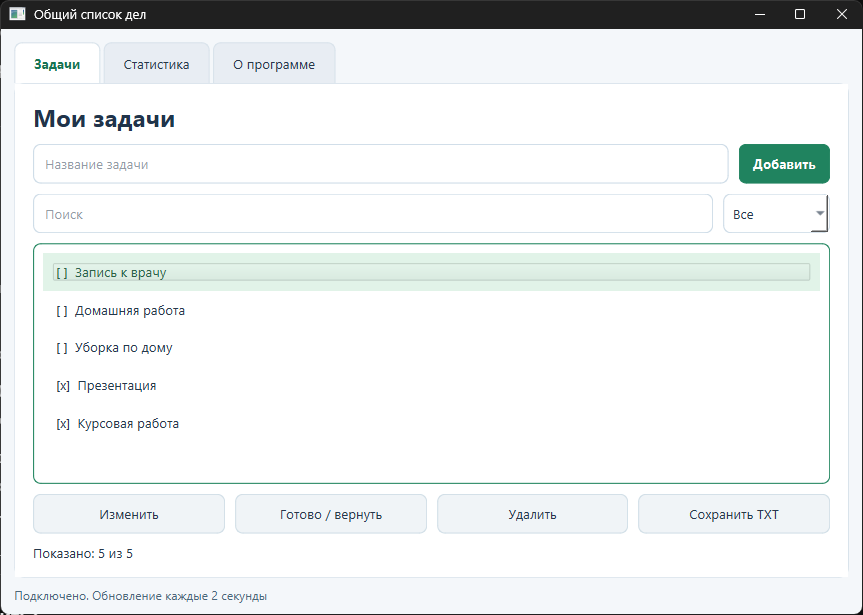
\includegraphics[width=.92\textwidth,height=.39\textheight,keepaspectratio]{figures/screenshots/tasks.png}
\caption{Окно приложения со списком задач}
\label{fig:taskwindow}
\end{figure}

Для поиска достаточно ввести часть названия. Фильтр «Все», «В работе» или «Выполнено» ограничивает видимые записи, но не изменяет данные на сервере. Перед названием показано [x] для выполненной задачи и [ ] для невыполненной. На снимке показаны пять задач, две из них отмечены выполненными. Среди записей есть «Запись к врачу», «Домашняя работа» и «Уборка по дому».

Редактирование выполняется через стандартный диалог ввода текста QInputDialog. Он открывается после выбора строки и нажатия кнопки «Изменить». На рисунке \ref{fig:editwindow} показано изменение названия первой задачи на «Запись к врачу в 19:00».

\begin{figure}[htbp]
\centering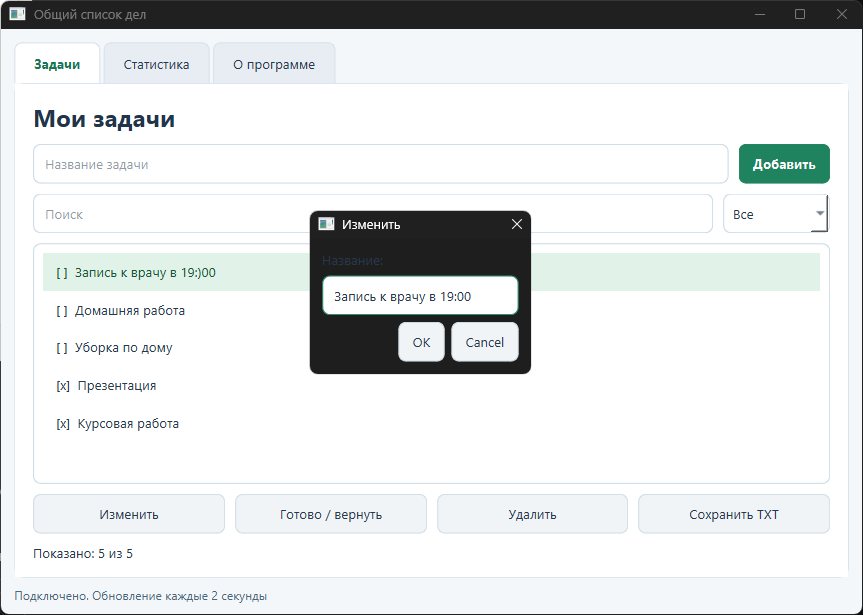
\includegraphics[width=.87\textwidth,height=.37\textheight,keepaspectratio]{figures/screenshots/edit.png}
\caption{Диалог изменения названия выбранной задачи}
\label{fig:editwindow}
\end{figure}

При пустом названии окно показывает подсказку. После подтверждения редактирования клиент отправляет запрос на сервер и перечитывает список. Если задача не выбрана, изменение не выполняется. Удаление также требует выбора записи и подтверждения действия.

На вкладке «Статистика» отображаются три числа: количество всех задач, задач в работе и выполненных. Шкала показывает долю выполненных. Значения рассчитываются из полученного списка; отдельного запроса к серверу для статистики нет. На рисунке \ref{fig:statswindow} показаны три блока статистики и шкала прогресса. В списке пять задач: три в работе и две выполнены, доля выполнения составляет 40\%.

\begin{figure}[htbp]
\centering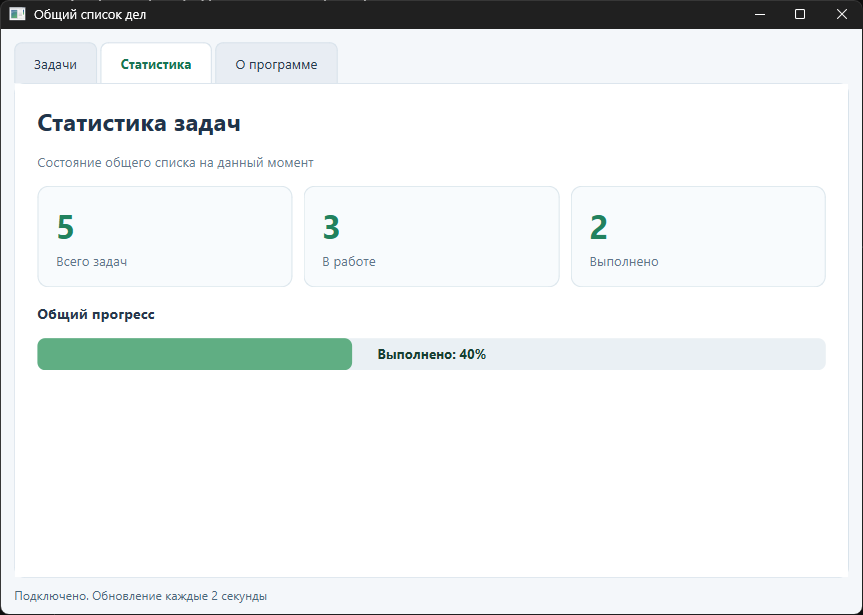
\includegraphics[width=.90\textwidth,height=.37\textheight,keepaspectratio]{figures/screenshots/stats.png}
\caption{Вкладка «Статистика» в работающем приложении}
\label{fig:statswindow}
\end{figure}

На вкладке «О программе» показаны назначение приложения, способ хранения данных, период обновления и адрес сервера (рисунок \ref{fig:aboutwindow}). Переключение между страницами выполнено с помощью QTabWidget \cite{qttabs}.

\begin{figure}[htbp]
\centering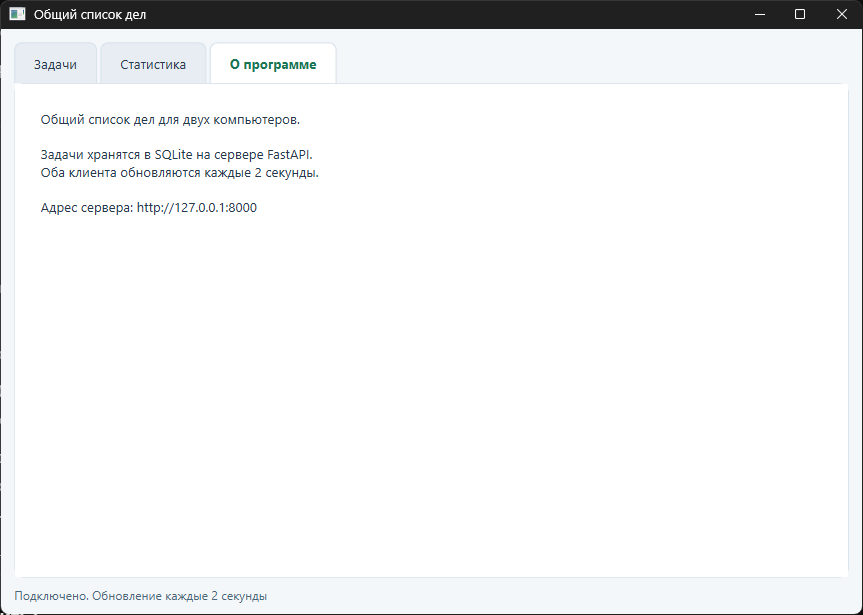
\includegraphics[width=.86\textwidth,height=.37\textheight,keepaspectratio]{figures/screenshots/about.png}
\caption{Вкладка «О программе» в работающем клиенте}
\label{fig:aboutwindow}
\end{figure}

Начальный размер окна составляет 780 на 530 пикселей. Элементы размещены в вертикальных и горизонтальных компоновщиках; при изменении размера окна область списка растягивается. Для вывода используется QListWidget: он позволяет связать строку с идентификатором задачи \cite{qtlist}. Благодаря этому одинаковые названия не мешают выбирать конкретную запись. Выделение сохраняется при обновлении списка, если выбранная задача ещё существует.

Для проверки совместной работы на одном компьютере запущены два отдельных окна клиента. После переименования задачи оба окна показывают запись «Запись к врачу в 19:00» (рисунок \ref{fig:twoclients}). Этот снимок подтверждает запуск двух экземпляров приложения и общее состояние списка на одном ПК; испытание связи между двумя физическими компьютерами проводится отдельно.

\begin{figure}[H]
\centering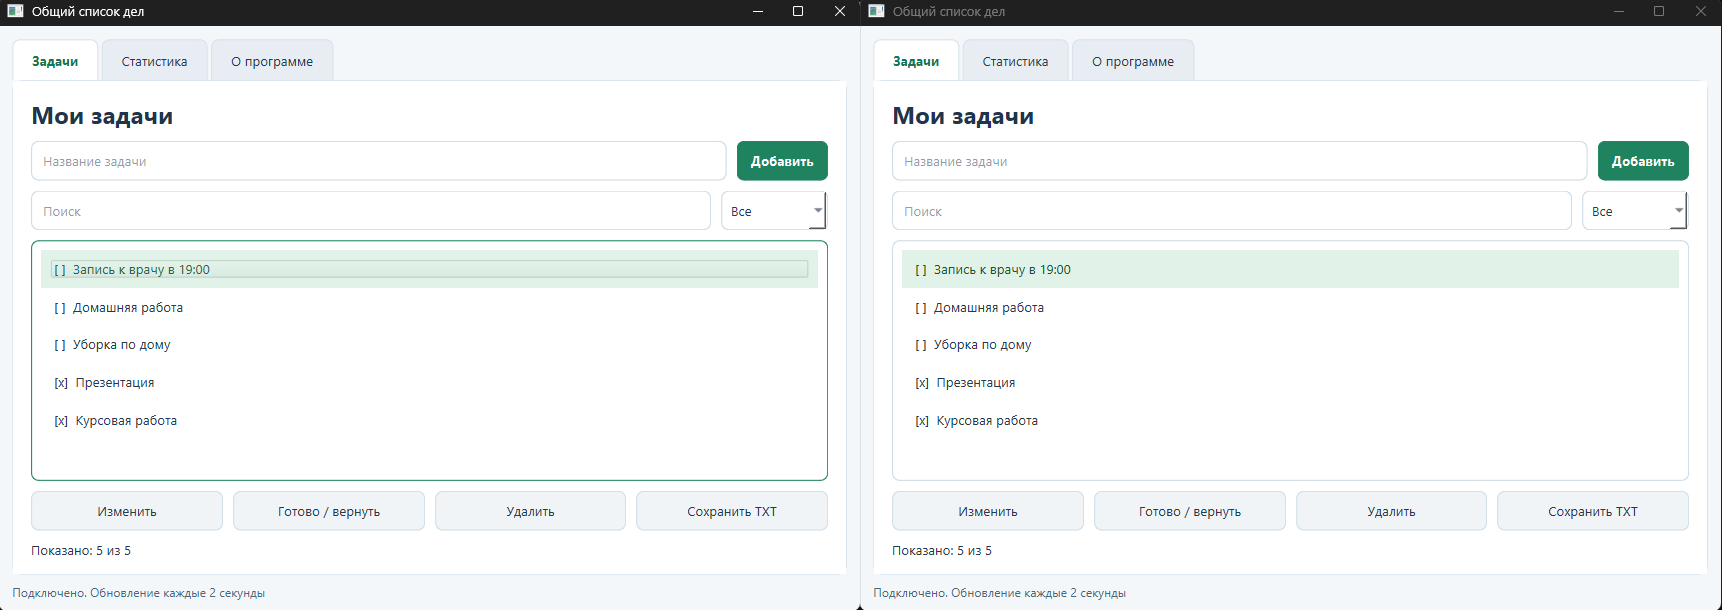
\includegraphics[width=.98\textwidth,height=.34\textheight,keepaspectratio]{figures/screenshots/two_clients.png}
\caption{Два клиента, запущенные на одном компьютере}
\label{fig:twoclients}
\end{figure}

Экспорт в TXT выполняется на компьютере пользователя. Программа записывает каждую задачу с отметкой [x] либо [ ] в отдельную строку. Используется кодировка UTF-8 с меткой BOM для корректного чтения русского текста в Блокноте Windows. На рисунке \ref{fig:exporttxt} показан файл, сохранённый из приложения и открытый в текстовом редакторе. Экспорт не меняет данные в SQLite.

\begin{figure}[H]
\centering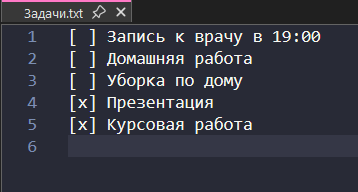
\includegraphics[width=.70\textwidth,height=.25\textheight,keepaspectratio]{figures/screenshots/export_txt.png}
\caption{Содержимое файла TXT после экспорта списка задач}
\label{fig:exporttxt}
\end{figure}

Если пользователь отменяет выбор файла, запись не выполняется. При ошибке сохранения появляется сообщение. При потере соединения с сервером клиент оставляет на экране последний полученный список и показывает в нижней строке состояние подключения. После восстановления связи список обновляется при следующем запросе.

\section{Проверка работы и сценарии приёмки}

Сервер проверялся на временной базе, не связанной с пользовательскими данными. Два экземпляра TestClient обращались к одной таблице и проверяли добавление, редактирование, переключение состояния, удаление и неверный ввод \cite{fastapitesting}. Затем тот же набор основных операций выполнялся через реально запущенный HTTP-сервер с двумя независимыми сеансами Requests. Проверки охватывали успешные операции, ошибочный ввод и сохранение записей. Эти испытания не использовали виджеты PySide6: проверялся обмен по HTTP и содержимое SQLite. Основные сценарии и ответы сервера приведены в таблице \ref{tab:autotests}.

\begin{table}[H]
\caption{Проверка основных HTTP-операций}
\label{tab:autotests}
\small\centering\renewcommand{\arraystretch}{1.22}
\begin{tabularx}{\textwidth}{|L{10mm}|Y|L{28mm}|}
\hline
№ & Проверяемое действие & Результат \\
\hline
1 & Получение пустого списка до добавления & HTTP 200; пустой список \\
\hline
2 & Создание задачи с русским названием & HTTP 200 \\
\hline
3 & Чтение новой задачи вторым тестовым клиентом & Запись найдена \\
\hline
4 & Редактирование названия и чтение первым клиентом & Новое название получено \\
\hline
5 & Изменение состояния и чтение первым клиентом & \texttt{done = true} \\
\hline
6 & Отклонение названия из пробелов & HTTP 400 \\
\hline
7 & Ошибка для отсутствующего идентификатора & HTTP 404 \\
\hline
8 & Удаление и повторное чтение & Запись отсутствует \\
\hline
9 & Открытие документации API & HTTP 200 \\
\hline
10 & Перезапуск HTTP-сервера с тем же файлом базы & Данные сохранены \\
\hline
\end{tabularx}
\end{table}

В таблице приведены операции серверной части. Поиск, фильтр, статистика и экспорт в TXT выполняются в клиентском окне и проверяются отдельно на Windows-ПК.

Один из сценариев включал следующую последовательность действий. Сначала сервер возвращает пустой список. Первый тестовый клиент отправляет название «Подготовить курсовую», после чего второй читает список и получает эту задачу. Второй клиент исправляет название и меняет состояние задачи на выполненное, а первый получает оба изменения при следующем чтении. После удаления оба видят пустой перечень. В этом примере проверяется совместное использование базы, а не скорость передачи данных.

Помимо основных операций проверена обработка неправильных запросов. В таблице \ref{tab:edgecases} приведены результаты повторной проверки, выполненной на временной базе без пользовательских данных.

\begin{table}[htbp]
\caption{Результаты проверки входных данных и запросов}
\label{tab:edgecases}
\small\centering\renewcommand{\arraystretch}{1.2}
\begin{tabularx}{\textwidth}{|L{47mm}|L{41mm}|Y|}
\hline
Проверяемое условие & Запрос & Фактический ответ \\
\hline
Название из пробелов & POST /tasks & HTTP 400 \\
\hline
Название из 121 символа & POST /tasks & HTTP 400 \\
\hline
Перевод строки и табуляция & POST /tasks & HTTP 400 \\
\hline
Несуществующий идентификатор & PATCH /tasks/999999 & HTTP 404 \\
\hline
Пустое название при редактировании & PATCH /tasks/1/title & HTTP 400 \\
\hline
Удаление отсутствующей задачи & DELETE /tasks/999999 & HTTP 404 \\
\hline
Название с апострофом & POST /tasks & HTTP 200, запись создана \\
\hline
Повторение названия & POST /tasks & HTTP 200, отдельная запись \\
\hline
\end{tabularx}
\end{table}

Проверки серверной части включали правильный ввод, ошибочные запросы, редактирование, отметки выполнения, удаление, получение изменений вторым HTTP-клиентом и сохранение SQLite после остановки сервера. В ходе проверки в Windows получены снимки главного экрана, статистики, редактирования, информационной вкладки, двух открытых клиентов и экспортированного текстового файла. Два окна работали на одном компьютере; проверка сетевого соединения между двумя физическими ПК остаётся отдельным сценарием из приложения Б.

\section{Ограничения программы}

Приложение не рассчитано на работу в публичной сети. На сервере отсутствуют вход пользователей и распределение прав. HTTP-запросы не шифруются, поэтому сервер следует запускать в доверенной локальной сети, не открывая порт для подключения из интернета.

При потере связи клиент оставляет на экране последний полученный список и сообщает, что связь с сервером отсутствует. Неотправленные действия не сохраняются. Текст новой задачи остаётся в поле ввода, чтобы пользователь мог повторить отправку после восстановления соединения. Следующий успешный опрос перечитает список.


\conclusion
Подготовлено приложение, в котором два настольных клиента обращаются к общему списку задач. Данные находятся в базе SQLite на компьютере-сервере; пользователям не приходится копировать файлы между устройствами.

Реализованы добавление, редактирование и удаление задач, переключение отметки выполнения, поиск и фильтрация полученного списка, а также его сохранение в TXT. В окне PySide6 три страницы: задачи, статистика и сведения о программе. Клиент проверяет обновления через FastAPI с периодом две секунды.

Проверены редактирование названий, передача изменений между независимыми HTTP-клиентами, неверный ввод и сохранение записей после перезапуска сервера. В Windows открыты два окна клиента с общим списком, проверены вкладка статистики, редактирование и экспорт TXT. Испытание взаимодействия между двумя физическими ПК не проводилось; порядок такой проверки приведён в приложении Б.

Для работы обоих клиентов требуется доступный компьютер-сервер. При отключении сети новые действия не сохраняются и должны быть повторены после восстановления соединения. При дальнейшем развитии программы сетевые запросы можно вынести из графического потока, чтобы окно не задерживалось при ожидании ответа.
\clearpage
\renewcommand{\bibname}{Список использованных источников}
\addcontentsline{toc}{chapter}{Список использованных источников}
\begingroup
\Urlmuskip=0mu plus 1mu
\urlstyle{same}
\raggedright
\begin{thebibliography}{99}
\bibitem{zaramenskikh} Зараменских Е.\,П. Проектирование информационных систем : учебник и практикум для вузов. - 2-е изд. - Москва : Юрайт, 2025. - 119 с. - ISBN 978-5-534-21418-5. - URL: \url{https://urait.ru/bcode/571331} (дата обращения: 04.11.2026).
\bibitem{chistov} Чистов Д.\,В., Мельников П.\,П., Золотарюк А.\,В., Ничепорук Н.\,Б. Проектирование информационных систем : учебник и практикум для вузов. - 2-е изд., перераб. и доп. - Москва : Юрайт, 2025. - 273 с. - ISBN 978-5-534-20361-5. - URL: \url{https://urait.ru/bcode/560485} (дата обращения: 04.11.2026).
\bibitem{polupanov} Полупанов Д.\,В., Абдюшева С.\,Р., Ефимов А.\,М. Программирование в Python 3 : учебное пособие. - Уфа : БашГУ, 2020. - 164 с. - ISBN 978-5-7477-5230-6. - URL: \url{https://e.lanbook.com/book/179915} (дата обращения: 04.11.2026).
\bibitem{yantsev} Янцев В.\,В. Web-программирование на Python : учебное пособие для вузов. - Санкт-Петербург : Лань, 2022. - 180 с. - ISBN 978-5-8114-9461-3. - URL: \url{https://e.lanbook.com/book/233264} (дата обращения: 04.11.2026).
\bibitem{prokhorenok} Прохоренок Н.\,А., Дронов В.\,А. Python 3 и PyQt 6. Разработка приложений. - Санкт-Петербург : БХВ-Петербург, 2023. - 832 с. - ISBN 978-5-9775-1706-5. - URL: \url{https://library.cbr.ru/catalog/lib/books/404707/} (дата обращения: 04.11.2026).
\bibitem{mdnhttp} MDN Web Docs. Обзор протокола HTTP [Электронный ресурс]. - URL: \url{https://developer.mozilla.org/ru/docs/Web/HTTP/Guides/Overview} (дата обращения: 04.11.2026).
\bibitem{pythonsqlite} Python Software Foundation. sqlite3 - DB-API 2.0 interface for SQLite databases [Электронный ресурс]. - URL: \url{https://docs.python.org/3/library/sqlite3.html} (дата обращения: 04.11.2026).
\bibitem{sqlitecreate} SQLite. CREATE TABLE [Электронный ресурс]. - URL: \url{https://www.sqlite.org/lang_createtable.html} (дата обращения: 04.11.2026).
\bibitem{fastapifirst} FastAPI. First Steps [Электронный ресурс]. - URL: \url{https://fastapi.tiangolo.com/tutorial/first-steps/} (дата обращения: 04.11.2026).
\bibitem{fastapibody} FastAPI. Request Body [Электронный ресурс]. - URL: \url{https://fastapi.tiangolo.com/tutorial/body/} (дата обращения: 04.11.2026).
\bibitem{fastapitesting} FastAPI. Testing [Электронный ресурс]. - URL: \url{https://fastapi.tiangolo.com/tutorial/testing/} (дата обращения: 04.11.2026).
\bibitem{qtdocs} Qt Company. Qt for Python - Documentation [Электронный ресурс]. - URL: \url{https://doc.qt.io/qtforpython-6/} (дата обращения: 04.11.2026).
\bibitem{qttabs} Qt Company. PySide6.QtWidgets.QTabWidget [Электронный ресурс]. - URL: \url{https://doc.qt.io/qtforpython-6/PySide6/QtWidgets/QTabWidget.html} (дата обращения: 04.11.2026).
\bibitem{qtlist} Qt Company. PySide6.QtWidgets.QListWidget [Электронный ресурс]. - URL: \url{https://doc.qt.io/qtforpython-6/PySide6/QtWidgets/QListWidget.html} (дата обращения: 04.11.2026).
\bibitem{qtimer} Qt Company. PySide6.QtCore.QTimer [Электронный ресурс]. - URL: \url{https://doc.qt.io/qtforpython-6/PySide6/QtCore/QTimer.html} (дата обращения: 04.11.2026).
\bibitem{requestsquick} Requests. Quickstart [Электронный ресурс]. - URL: \url{https://requests.readthedocs.io/en/latest/user/quickstart/} (дата обращения: 04.11.2026).
\bibitem{rfchttp} Fielding R., Nottingham M., Reschke J. HTTP Semantics. RFC 9110. - IETF, 2022. - URL: \url{https://datatracker.ietf.org/doc/html/rfc9110} (дата обращения: 04.11.2026).
\bibitem{rfcjson} Bray T. The JavaScript Object Notation (JSON) Data Interchange Format. RFC 8259. - IETF, 2017. - URL: \url{https://datatracker.ietf.org/doc/html/rfc8259} (дата обращения: 04.11.2026).
\bibitem{owaspvalidation} OWASP Cheat Sheet Series. Input Validation Cheat Sheet [Электронный ресурс]. - URL: \url{https://cheatsheetseries.owasp.org/cheatsheets/Input_Validation_Cheat_Sheet.html} (дата обращения: 04.11.2026).
\bibitem{gostflow} ГОСТ 19.701-90 (ИСО 5807-85). Единая система программной документации. Схемы алгоритмов, программ, данных и систем. Обозначения условные и правила выполнения. - Росстандарт. - URL: \url{https://protect.gost.ru/gost/details/0c85e066-f89e-433d-a6d3-b7f746bd0c7c} (дата обращения: 04.11.2026).
\end{thebibliography}
\endgroup

\clearpage
\chapter*{Приложение А}
\phantomsection\addcontentsline{toc}{chapter}{Приложение А. Примеры входных и выходных данных}
\begin{center}\textbf{Примеры входных и выходных данных}\end{center}

В таблице \ref{tab:app-examples} приведены примеры действий в интерфейсе. Входными данными служат название задачи и выбор записи или команды. Результатом становится изменение списка, статистики или сообщение пользователю.

\begingroup
\renewcommand{\thetable}{А.\arabic{table}}
\setcounter{table}{0}
\begin{table}[htbp]
\caption{Примеры действий пользователя и результатов}
\label{tab:app-examples}
\small\centering\renewcommand{\arraystretch}{1.28}
\begin{tabularx}{\textwidth}{|L{39mm}|Y|Y|}
\hline
Действие & Входные данные & Ожидаемый результат \\
\hline
Добавление & «Сдать практическую работу» & Новая строка в общем списке \\
\hline
Повторное чтение & Открытие списка на втором ПК & Та же строка появляется у второго клиента \\
\hline
Отметка выполнения & Выбрана добавленная задача & Перед названием показано [x] \\
\hline
Изменение названия & Выбрана задача «Подготовить курсовую» & Новое название сохраняется в базе \\
\hline
Поиск & Введено слово «курсовую» & Отображаются записи с совпадением \\
\hline
Фильтр & Выбрано «Выполнено» & Показаны только выполненные задачи \\
\hline
Статистика & Три задачи, одна выполнена & Доля выполнения составляет 33\% \\
\hline
Экспорт в TXT & Две задачи с разными отметками & В выбранном файле записаны обе задачи \\
\hline
Возврат в работу & Выбрана выполненная задача & Перед названием показано [ ] \\
\hline
Неверный ввод & Пустая строка или пробелы & Показана подсказка; запись не создаётся \\
\hline
Удаление & Выбрана существующая задача & Строка исчезает из общего списка \\
\hline
Отсутствие связи & Компьютер-сервер выключен & В строке состояния указано, что соединение отсутствует \\
\hline
\end{tabularx}
\end{table}
\endgroup



\chapter*{Приложение Б}
\phantomsection\addcontentsline{toc}{chapter}{Приложение Б. Порядок проверки на двух компьютерах}
\begin{center}\textbf{Порядок проверки на двух компьютерах}\end{center}

Для демонстрации на одном компьютере запускают \path{START.bat}: открывается сервер и два независимых окна клиента. Для проверки двух физических ПК на первом запускают \path{SERVER_ONLY.bat}, а на втором \path{CLIENT_OTHER_PC.bat} и вводят локальный IPv4-адрес первого компьютера.

При проверке на двух физических ПК оба компьютера должны находиться в одной локальной сети. Для определения IPv4-адреса на первом ПК выполняют команду \texttt{ipconfig}. Если второй компьютер не подключается, проверяют адрес сервера и правила брандмауэра для порта 8000.

После подключения на первом ПК создают задачу «Подготовить курсовую». На втором ПК проверяют появление записи после обновления списка. Затем исправляют название, меняют отметку выполнения и проверяют изменение на первом ПК. На каждом клиенте проверяют поиск, фильтр и показатели страницы «Статистика». Также нажимают «Сохранить TXT», выбирают файл и открывают его в Блокноте Windows. В завершение удаляют задачу. Для проверки сохранения создают новую запись, перезапускают сервер и убеждаются, что запись осталась в списке. Для проверки ошибки соединения временно останавливают сервер, ждут сообщения об отсутствии связи, затем запускают сервер снова и проверяют восстановление списка.

\vfill
\noindent Дата окончания курсового проекта: \rule{53mm}{0.4pt}\\[6mm]
\noindent Подпись автора: \rule{77mm}{0.4pt}

\end{document}
